\documentclass{article}

\usepackage[utf8]{inputenc}
\usepackage[russian]{babel}
\usepackage[a4paper, margin=1in]{geometry}
\usepackage{graphicx}
\usepackage{amsmath}
\usepackage{wrapfig}
\usepackage{multirow}
\usepackage{mathtools}
\usepackage{pgfplots}
\usepackage{pgfplotstable}
\usepackage{setspace}
\usepackage{changepage}
\usepackage{caption}
\usepackage{csquotes}
\usepackage{hyperref}
\usepackage{listings}

\pgfplotsset{compat=1.18}
\hypersetup{
  colorlinks = true,
  linkcolor  = blue,
  filecolor  = magenta,      
  urlcolor   = darkgray,
  pdftitle   = semt-report-vcs-smirnov-shinakov,
}

\definecolor{codegreen}{rgb}{0,0.6,0}
\definecolor{codegray}{rgb}{0.5,0.5,0.5}
\definecolor{codepurple}{rgb}{0.58,0,0.82}
\definecolor{backcolour}{rgb}{0.99,0.99,0.99}

\lstdefinestyle{codestyle}{
  backgroundcolor=\color{backcolour},   
  commentstyle=\color{codegreen},
  keywordstyle=\color{magenta},
  numberstyle=\tiny\color{codegray},
  stringstyle=\color{codepurple},
  basicstyle=\ttfamily\footnotesize,
  breakatwhitespace=false,         
  breaklines=true,                 
  captionpos=b,                    
  keepspaces=true,                 
  numbers=left,                    
  numbersep=5pt,                  
  showspaces=false,                
  showstringspaces=false,
  showtabs=false,                  
  tabsize=2
}

\lstset{style=codestyle}
\begin{document}

\begin{titlepage}
  \begin{center}
    \begin{spacing}{1.4}
      \large{Университет ИТМО} \\
      \large{Факультет программной инженерии и компьютерной техники} \\
    \end{spacing}
    \vfill
    \textbf{
      \huge{Методы и средства программной инженерии.} \\
      \huge{Лабораторная работа №2.} \\
      \huge{Системы контроля версий} \\
    }
  \end{center}
  \vfill
  \begin{center}
    \begin{tabular}{r l}
      Смирнов Виктор Игоревич  & P32131 \\
      Шиняков Артём Дмитриевич & R32372 \\
      Вариант                  & 1009   \\
    \end{tabular}
  \end{center}
  \vfill
  \begin{center}
    \begin{large}
      2023
    \end{large}
  \end{center}
\end{titlepage}

\tableofcontents

\section{Задание}

Сконфигурировать в своём домашнем каталоге репозитории svn и git 
и загрузить в них начальную ревизию файлов с исходными кодами 
(в соответствии с выданным вариантом).

Воспроизвести последовательность команд для систем контроля версий 
svn и git, осуществляющих операции над исходным кодом, приведённые 
на блок-схеме.

При составлении последовательности команд необходимо учитывать 
следующие условия:
\begin{enumerate}
    \item Цвет элементов схемы указывает на пользователя, совершившего 
          действие (красный - первый, синий - второй).
    \item Цифры над узлами - номер ревизии. Ревизии создаются последовательно.
    \item Необходимо разрешать конфликты между версиями, если они возникают.
\end{enumerate}

\begin{figure}[h]
    \centering
    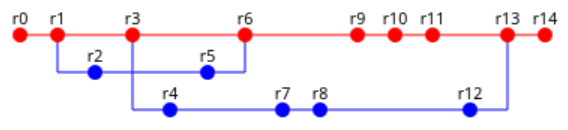
\includegraphics[
        width=\linewidth / 2
    ]{../res/history.png}
    \caption{История ревизий репозитория}
    \label{fig:history}
\end{figure}


\section{Взаимодействие с репозиторием через SVN}

\lstinputlisting[language=Bash]{../../ci/svn/main.sh}
\lstinputlisting[language=Bash]{../../ci/svn/r_init.sh}
\lstinputlisting[language=Bash]{../../ci/svn/r0.sh}
\lstinputlisting[language=Bash]{../../ci/svn/r1.sh}
\lstinputlisting[language=Bash]{../../ci/svn/r2.sh}
\lstinputlisting[language=Bash]{../../ci/svn/r3.sh}
\lstinputlisting[language=Bash]{../../ci/svn/r4.sh}
\lstinputlisting[language=Bash]{../../ci/svn/r5.sh}
\lstinputlisting[language=Bash]{../../ci/svn/r6.sh}
\lstinputlisting[language=Bash]{../../ci/svn/r7.sh}
\lstinputlisting[language=Bash]{../../ci/svn/r8.sh}
\lstinputlisting[language=Bash]{../../ci/svn/r9.sh}
\lstinputlisting[language=Bash]{../../ci/svn/r10.sh}
\lstinputlisting[language=Bash]{../../ci/svn/r11.sh}
\lstinputlisting[language=Bash]{../../ci/svn/r12.sh}
\lstinputlisting[language=Bash]{../../ci/svn/r13.sh}
\lstinputlisting[language=Bash]{../../ci/svn/r14.sh}
\lstinputlisting[language=Bash]{../../ci/svn/lib/head.sh}
\lstinputlisting[language=Bash]{../../ci/svn/lib/dsl.sh}

\section{Вывод}

Выполнив данную лабораторную работу мы научились 
использовать базовые функции таких известных систем
контроля версий как git и svn. Оба пакета программного
обеспечения предоставляют весь необходимый функционал
для удобного использования, но управляются пользователем
по-разному, что делает одну СКВ предпочтительнее другой
в зависимости от сложившейся ситуации. Например, интерфейс
системы контроля версий git немного проще svn и предлагает
более лаконичную (не факт) схему работы с репозиторием. A 
svn в свою очередь может предложить очень удобный механизм
частичного монтажа поддиректорий репозитория, такая 
функциональность может быть полезна, когда мы имеем дело
с монорепозиториями и не хотим видеть сразу все содержимое
большого проекта.

\end{document}
